\chapter{قابلية الإشتقاق في $\R^n$}
\thispagestyle{empty}
\newpage
\section{المشتقة الجزئية}
\begin{definition}
    لتكن $f:\cbracket{x_1}\times\dots\times\cbracket{x_{j-1}}\times[a,b]\times\cbracket{x_{j+1}}\times\dots\times\cbracket{x_n}\to\R$ ، سوف نرمز للدالة التالية
    \[
    g(t):=f(x_1,\dots,x_{j-1},t,x_{j+1},\dots,x_n),\quad t\in[a,b]
    \]
    بالرمز $f(x_1,\dots,x_{j-1},\cdot,x_{j+1},\dots,x_n)$. إذا كانت $g$ قابلة للإشتقاق عند بعض $t_0\in(a,b)$ ، إذن المشتقة الجزئية (أو المشتقة الجزئية من الرتبة الأولى) إلى الدالة $f$ عند \\$(x_1,\dots,x_{j-1},t_0,x_{j+1},\dots,x_n)$ بالنسبة إلى $x_{j}$ تعرف بالشكل
    \[
    \pder{f}{x_j}(x_1,\dots,x_{j-1},t_0,x_{j+1},\dots,x_n):=g^{\prime}(t_0)
    \]
 \end{definition}
    كذلك نرمز لهذه المشتقة الجزئية بالرمز $f_{x_j}(x_1,\dots,x_{j-1},t_0,x_{j+1},\dots,x_n)$. إذن من تعريف المشتقة من الفصل الأول أن المشتقة الجزئية $f_{x_{j}}$ موجودة عند نقطة $\A$ إذا وفقط إذا كانت الغاية
\[
\pder{f}{x_j}(\A):=\lim\limits_{h\rightarrow 0}\frac{f(\A+h\e_j)-f(\A)}{h}
\]
موجودة. سوف نوسع مفهوم المشتقة الجزئية إلى دوال إتجاهية بالطريقة التالية. أفرض أن $\A=(a_1,\dots,a_n)\in\R^n$ و $\f=(f_1,\dots,f_m):\cbracket{a_1}\times\dots\times\cbracket{a_{j-1}}\times I\times\cbracket{a_{j+1}}\times\dots\times\cbracket{a_n}\rightarrow \R^m$ حيث $j\in\cbracket{1,2,\dots,n}$ و $I$ فترة مفتوحة تحوي $a_j$. اذا كان لكل $k=1,2,\dots,m$ المشتقة الجزئية من الرتبة الأولى $\partial f_k/\partial x_j$ موجودة عند $\A$ عندها نعرف المشتقة الجزئية من الرتبة الأولى للدالة $\f$ بالنسبة إلى $x_j$ لتكون الدالة الإتجاهية
\[
\f_{x_j}(\A):=\pder{f}{x_j}(\A):=\pbracket{\pder{f_1}{x_j}(\A),\dots,\pder{f_m}{x_j}(\A)}
\]
المشتقات الجزئية من الرتب العليا تعرف بالتكرار. على سبيل المثال المشتقة الجزئية من الرتبة الثانية للدالة $\f$ بالنسبة إلى $x_j$ و $x_k$ تعرف بالصورة التالية عندما تكون موجودة
\[
\f_{x_jx_k}:=\pder{^2\f}{x_k\partial x_j}:=\pder{}{x_k}\pbracket{\pder{\f}{x_j}}
\]
المشتقات الجزئية من الرتبة الثانية تسمى مختلطة عندما $j\neq k$.

\section{الفضاء $C^{\infty}$}
\begin{definition}
    لتكن $V$ مجموعة غير خالية. مجموعة جزئية مفتوحة من $\R^n$ ولتكن $\f:V\to\R^m$ دالة و $p\in\N$ 
    \begin{enumerate}
        \item[.i] يقال أن $\f$ تنتمي إلى $C^p$ على $V$ إذا وفقط إذا كانت كل مشتقة جزئية من الرتبة $k\leq p$ موجودة و مستمرة على $V$.

        \item[.ii] يقال أن $\f$ تنتمي إلى $C^{\infty}$ على $V$ إذا وفقط إذا كانت $\f$ تنتمي إلى $C^p$ على $V$ لكل $p\in\N$.
    \end{enumerate}
\end{definition}

\begin{note}
    للتبسيط سوف ننص كل النتائج و المبرهنات في هذا الفصل من أجل $n=2$ و $m=1$ مستخدمين $x$ من أجل $x_1$ و $y$ من أجل $x_2$.
\end{note}

\begin{note}
    بما أن المشتقات الجزئية هي من الأساس مفاهيم أحادية البعد، لذلك كل نتيجة تخص المشتقة أحادية البعد تحتوي معلومات حول المشتقات الجزئية ، وهنا مثالين :
    \begin{enumerate}
    \item بإستخدام قاعدة الضرب (مبرهنة \ref{derivatives_rules}) ، إذا كانت $f_x$ و $g_x$ موجودة، إذن
    \[
    \pder{}{x}(f\cdot g)=f\pder{g}{x}+g\pder{f}{x}
    \]

    \item بإستخدام مبرهنة القيمة المتوسطة (مبرهنة \ref{mean_value_theorem}). إذا كانت $f(\cdot,y)$ مستمرة على الفترة $[a,b]$ والمشتقة الجزئية $f_x(\cdot,y)$ موجودة على $(a,b)$ ، إذن يوجد عدد $c\in(a,b)$ (الذي من الممكن أن يعتمد على $y$) حيث
\[
f(b,y)-f(a,y)=(b-a)\pder{f}{x}(c,y)
\]
    \end{enumerate}
\end{note}

\begin{theorem}
\label{mixed_partial_equation}
    افرض ان $V$ مجموعة مفتوحة في $\R^2$ وأن $(a,b)\in V$ نقطة ، وأن $f:V\to\R$ دالة ، إذا كانت $f\in C^1(V)$ و واحدة من المشتقات المختلطة من الرتبة الثانية للدالة $f$ موجودة على $V$ ومستمرة عند النقطة $(a,b)$. إذن المشتقة المختلطة من الرتبة الثانية الأخرى موجودة عند $(a,b)$ و
\[
\pder{^2f}{y\partial x}(a,b)=\pder{^2f}{x\partial y}(a,b)
\]
\end{theorem}

المثال التالي يبين أن المبرهنة \ref{mixed_partial_equation} خاطئة إذا كانت الاستمرارية غير متحققة بالنسبة إلى المشتقة المختلطة من الرتبة الثانية.

\begin{example}
    أثبت أن الدالة
\[
f(x,y)=\begin{cases}
    xy\pbracket{\dfrac{x^2-y^2}{x^2+y^2}}&, (x,y)\neq(0,0)\\
    0&, (x,y)=(0,0)
\end{cases}
\]
تنتمي إلى $C^1(\R^2)$ وأن كلا المشتقتين المختلطتين من الرتبة الثانية موجودة على $\R^2$. ولكنها لا تتبادل عند $(0,0)$ ، أي أن $f_{xy}(0,0)\neq f_{yx}(0,0)$.
\end{example}

\begin{myproof}
    عندما $(x,y)\neq(0,0)$ و بإستخدام قاعدتي الضرب و القسمة أحادية البعد ، نحصل على
    \begin{align*}
        \pder{f}{x}(x,y)&=xy\pder{}{x}\pbracket{\frac{x^2-y^2}{x^2+y^2}}+\pder{}{x}(xy)\pbracket{\frac{x^2-y^2}{x^2+y^2}}\\
        &=xy\pbracket{\frac{4xy^2}{(x^2+y^2)^2}}+y\pbracket{\frac{x^2-y^2}{x^2+y^2}}
    \end{align*}
    بما أن $2\abs{xy}\leq x^2+y^2$ لدينا $\abs{f_x(x,y)}\leq 2\abs{y}$ وبالتالي $f_x(x,y)\to0$ عندما $(x,y)\to(0,0)$. من الناحية الأخرى بإستخدام التعريف
    \[
    \pder{f}{x}(0,y)=\lim\limits_{h\to0}y\pbracket{\frac{h^2-y^2}{h^2+y^2}}=-y
    \]
    لكل $y\in\R$ ، إذن $f_x(0,0)=0$ هذا يثبت أن $f_x$ موجودة و مستمرة على $\R^2$ مع القيمة $-y$ عند $(0,y)$. وبأسلوب مشابه نثبت أن $f_y$ موجودة ومستمرة على $\R^2$ مع القيمة $x$ عند $(x,0)$.\\
    وهذا يعني أن المشتقات الجزئية المختلطة من الرتبة الثانية موجودة على $\R^2$ ولكن
    \[
    \pder{^2f}{y\partial x}(0,0)=-1\neq 1=\pder{^2f}{x\partial y}(0,0)
    \]
\end{myproof}

\begin{example}
أحسب كل المشتقات الجزئية المختلطة من الرتبة الثانية لكل الدوال الآتية وتحقق من تساويها.
\begin{tasks}[label=\arabic*),label-width=14pt](3)
    \task $f(x,y)=y^2e^x$
    \task $f(x,y)=\sin(xy)$
    \task $f(x,y)=\dfrac{x-2y}{1-2y^2}$
\end{tasks}
\end{example}

\begin{solution}
    \begin{tasks}[label=\arabic*),label-width=14pt]
    \task $f(x,y)=y^2e^x$
    \[
    f_x=y^2e^x\Rightarrow f_{xy}=2ye^x
    \]
    و
\[
f_y=2ye^x\Rightarrow f_{yx}=2ye^x
\]
إذن $f_{xy}=f_{yx}$.
    \task $f(x,y)=\sin(xy)$
    \[
    f_x=y\cos{(xy)}\Rightarrow f_{xy}=\cos{(xy)}-xy\sin{(xy)}
    \]
و
\[
f_y=x\cos{(xy)}\Rightarrow f_{yx}=\cos{xy}-xy\sin{(xy)}
\]
إذن $f_{xy}=f_{yx}$. 

    \task $f(x,y)=\dfrac{x-2y}{1-2y^2}$
\[
f_x=\frac{1}{1-2y^2}\Rightarrow f_{xy}=\frac{4y}{(1-2y^2)^2}
\]
و
\begin{align*}
f_y&=\frac{(1-2y^2)(-2)-(x-2y)(-4y)}{(1-2y^2)^2}\\[7pt]
&=\frac{-2+4y^2+4xy-8y^2}{(1-2y^2)^2}\\[7pt]
&=\frac{4xy-4y^2-2}{(1-2y^2)^2} \Rightarrow f_{yx}=\frac{4y}{(1-2y^2)^2}
\end{align*}
إذن $f_{xy}=f_{yx}$.
    \end{tasks}
\end{solution}

\begin{example}
    أحسب $f_x$ للدالة الآتية وحدد أين تكون مستمرة 
    \[
    f(x,y)=\begin{cases}
        \dfrac{x^6+y^6}{x^3+y^3} &,(x,y)\neq(0,0)\\
        0 &, (x,y)=(0,0)
    \end{cases}
    \]
\end{example}

\begin{solution}
    عندما $(x,y)\neq(0,0)$
    \begin{align*}
        f_x(x,y)&=\pder{}{x}\pbracket{\frac{x^6+y^6}{x^3+y^3}}\\[8pt]
        &=\frac{(x^3+y^3)(6x^5)-(x^6+y^6)(3x^2)}{(x^3+y^3)^2}\\[8pt]
        &=\frac{3x^8+6x^5y^3-3x^2y^6}{(x^3+y^3)^2}
    \end{align*}
    وهذه المشتقة مستمرة عند كل $(x,y)\neq(0,0)$. الآن نناقش استمرارية المشتقة $f_x$ عند النقطة $(0,0)$. حسب التعريف لدينا
    \[
    f_x(0,0)=\lim\limits_{h\to0}\frac{f(h,0)-f(0,0)}{h}=\lim\limits_{h\to0}\frac{\frac{h^6+0}{h^3+0}-0}{h}=\lim\limits_{h\to0} h^2=0
    \]
    الآن نلاحظ عندما $(x,y)\to(0,0)$ 
    \[
    3x^8+6x^5y^3-3x^2y^6\leq 3x^2(x^6+2x^3y^3+y^6)=3x^2(x^3+y^3)^2
    \]
    إذن
    \[
    \abs{f_x(x,y)}\leq \frac{3x^2(x^3+y^3)^2}{(x^3+y^3)^2}=3x^2\longrightarrow0
    \]
    عندما $x\to0$. إذن $f_x$ مستمرة عند جميع نقاط $\R^2$.
\end{solution}

\section{تعريف قابلية الاشتقاق في $\R^n$}

\begin{definition}
    \label{def:differentiability_in_Rn}
    أفرض أن $\A\in\R^n$ وأن $V$ مجموعة مفتوحة تحوي $\A$. لتكن $\f:V\to\R^m$ دالة فإن
\begin{tasks}
    \task[.i] يقال بأن $\f$ قابلة للإشتقاق عند $\A$ إذا وفقط إذا وجدت $\T\in\Lap(\R^n:\R^m)$ بحيث أن الدالة 
    \[
    \epsilon(\h):=\f(\A+\h)-\f(\A)-\T(\h)
    \]
    تحقق $\epsilon(\h)/\norm{\h}\to0$ عندما $\h\to0$.
    \task[.ii] يقال بأن $\f$ قابلة للاشتقاق على مجموعة $E$ إذا وفقط إذا كانت $E$ مجموعة غير خالية و $\f$ قابلة للاشتقاق عند كل نقطة في $E$.
\end{tasks}
\end{definition}

\begin{theorem}
    إذا كانت $\f$ دالة إتجاهية قابلة للإشتقاق عند $\A$ ، إذن $\f$ دالة مستمرة عند $\A$.
\end{theorem}
\begin{myproof}
    افرض أن $\f$ دالة قابلة للاشتقاق عند $\A$. إذن بواسطة التعريف \ref{def:differentiability_in_Rn} يوجد تحويل خطي $\T\in\Lap(\R^n:\R^m)$ وعدد $\delta>0$ بحيث $\norm{\f(\A+\h)-\f(\A)-\T(\h)}\leq\norm{\h}$ لكل $\norm{\h}>\delta$. الآن بواسطة المتراجحة المثلثية وتعريف طول المتجه ، ينتج
\[
\norm{\f(\A+\h)-\f(\A)}\leq\norm{\T}\norm{\h}+\norm{\h}
\]
لكل $\norm{\h}>\delta$. بما أن $\norm{\T}$ عدد حقيقي منتهِ. نستنتج من مبرهنة الساندويتش بأن $\f(\A+\h)\to \f(\A)$ عندما $\h\to\Bzero$. بعبارة أخرى $\f$ مستمرة عند $\A$.
\end{myproof}

\begin{theorem}
    لتكن $\f$ دالة اتجاهية. إذا كانت $f$ قابلة للاشتقاق عند $\A$ إذن كل المشتقات الجزئية من الرتبة الأولى للدالة $\f$ موجودة عند $\A$. أبعد من ذلك فإن المشتقة الكلية للدالة $\f$ عند $\A$ تكون وحيدة وتحسب كالآتي
\[
D \f(\A)=\sbracket{\pder{f_i}{x_j}(\A)}_{m\times n}:=\begin{bmatrix}
    \pder{f_1}{x_1}(\A) & \dots & \pder{f_1}{x_n}(\A)\\
    \vdots & \ddots & \vdots\\
    \pder{f_m}{x_1}(\A) & \dots & \pder{f_m}{x_n}(\A)
\end{bmatrix}
\]
\end{theorem}
\begin{myproof}
    بما أن $\f$ قابلة للاشتقاق ، نعرف أنه توجد مصفوفة $B:=[b_{ij}]$ من الحجم $m\times n$ بحيث أن
    \begin{equation}
    \label{eq:thm_2}
    \frac{\f(\A+\h)-f(\A)-B\h}{\norm{\h}}\to\Bzero\quad\text{عندما}\quad \h\to\Bzero
    \end{equation}
    نحدد $1\leq j\leq n$ ونختار $\h=t\e_j$ لبعض $t>0$. بما أن $\norm{\h}=t$ لدينا 
    \[
    \frac{\f(\A+\h)-\f(\A)-B\h}{\norm{\h}}:=\frac{\f(\A+\h)-\f(\A)}{t}-B\e_j
    \]
    نأخذ الغاية عندما $t\to0^+$ و بإستخدام \eqref{eq:thm_2} وتعريف ضرب المصفوفات ، نحصل على
    \[
    \lim\limits_{t\to0^+}\frac{\f(\A+t\e_j)-\f(\A)}{t}=B\e_j=(b_{1j},b_{2j},\dots,b_{mj})
    \]
بأسلوب مشابه نثبت أن الغاية عندما $t\to0^-$ أيضاً تساوي $(b_{1j},b_{2j},\dots,b_{mj})$. بما أن الدالة الاتجاهية متقاربة إذا وفقط إذا كانت مركباتها متقاربة وبهذا ينتج أن المشتقة الجزئية من الرتبة الأولى لكل مركبة $f_i$ بالنسبة إلى $x_j$ موجودة عند $\A$ وتحقق
\[
\pder{f_i}{x_j}(\A)=b_{ij}
\]
لكل $i=1,2,\dots,m$. بالخصوص. لكل دالة $\f$ قابلة للإشتقاق عند $\A$ يوجد تحويل خطي وحيد $\T\in\Lap(\R^n:\R^m)$ تحقق التعريف \ref{def:differentiability_in_Rn} ويكون الاشتقاق التام (الكلي) بالشكل
\[
D\f(\A):=[b_{ij}]_{m\times n}=\sbracket{\pder{f_i}{x_j}(\A)}_{m\times n}
\]
\end{myproof}

\begin{note}
    الآن لدينا عدة طرق لمعرفة ما إذا كانت الدالة الاتحاهية $\f$ قابلة للاشتقاق عند نقطة $\A$. بالتأكيد تكون $\f$ قابلة للاشتقاق عند $\A$ إذا وجدت مصفوفة $B$ من حجم $m\times n$ بحيث
\[
\lim\limits_{\h\to\Bzero}\frac{\f(\A+\h)-\f(\A)-B\h}{\norm{\h}}=0
\]
إذا وفقط إذا
\[
\lim\limits_{\h\to\Bzero}\frac{\norm{\f(\A+\h)-\f(\A)-B\h}}{\norm{\h}}=0
\]
أو إذا وفقط إذا
\begin{equation}
    \label{eq:differentiability_second_eq}
\lim\limits_{\h\to\Bzero}\frac{\f(\A+\h)-\f(\A)-D\f(\A)(\h)}{\norm{\h}}=0
\end{equation}
\end{note}

\begin{note}
    أول شرطين يمكن تطبيقهما بدون حساب المشتقات الجزئية للدالة $\f$. أما الشرط الأخير ملموس أكثر ولكن يُطبق فقط في حالة قدرتنا على على حساب المشتقات الجزئية من الرتبة الأولى للدالة $\f$.
\end{note}

\begin{note}
    إذا كان $n=1$ أو $m=1$. المصفوفة $D\f$ تصبح متجهاً ويصبح لدينا عدة أشكال
    \begin{tasks}
    \task[(i]   إذا كان $n=1$ ، فإن
\[
D\f(\A)=\begin{bmatrix}
    f_1'(a)\\
    \vdots\\
    f_m'(a)
\end{bmatrix}
\]
في بعض الأحيان نستخدم تعبير المتجهات
\[
\f'(a):=(f_1'(a),\dots,f_m'(a)
\]

\task[(ii] إذا كانت $m=1$ ، فإن 
\[
D\f(\A)=\begin{bmatrix}\pder{f}{x_1}(\A)&\dots&\pder{f}{x_n}(\A)
\end{bmatrix}
\]
في بعض الأحيان نستخدم تعبير المتجهات
\[
\nabla \f(\A):=\pbracket{\pder{f}{x_1}(\A),\dots,\pder{f}{x_n}(\A)}
\]
حيث $\nabla\f$ يسمى إنحدار الدالة $\f$.
    \end{tasks}
\end{note}

\begin{theorem}
    لتكن $V$ مجموعة مفتوحة في $\R^n$ و $\A\in V$ ولتكن $\f:V\to\R^m$ دالة اتجاهية. إذا كانت كل المشتقات الجزئية من الرتبة الأولى للدالة $\f$ موجودة في $V$ ومستمرة عند $\A$ إذن $\f$ قابلة للإشتقاق عند $\A$.
\end{theorem}
\begin{myproof}
    بما أن الدالة تتقارب إذا وفقط إذا كانت كل مركباتها متقاربة إذن يمكننا فرض $m=1$ وبواسطة التعريف يكفي أن نثبت أن $f$ دالة حقيقية تمتلك مشتقات مستمرة من الرتبة الأولى في $V$ وبعدها 
    \[
    \lim\limits_{\h\to\Bzero}\frac{f(\A+\h)-f(\A)-\nabla f(\A)\cdot\h}{\norm{\h}}=0.
    \]
    لتكن $\A=(a_1,\dots,a_n)$ ونفرض أن $r>0$ صغيرة جداً بحيث $B_r(\A)\subset V$. نحدد $\h=(h_1,\dots,h_n)\neq\Bzero$. الآن بإستخدام مبرهنة القيمة المتوسطة \ref{mean_value_theorem} (أحادية البعد)، نستطيع أن نختار $c_j$ بين $a_j$ و $a_j+h_j$ بحيث
    \begin{align*}
    f(\A+\h)-f(\A)&=f(a_1+h_1,\dots,a_n+h_n)-f(a_1,a_2+h_2,\dots,a_n+h_n)\\
    &\phantom{=}+\dots+f(a_1,\dots,a_{n-1},a_n+h_n)-f(a_1,\dots,a_n)\\
    &=\sum_{j=1}^{n}h_j\pder{f}{x_j}(a_1,\dots,a_{j-1},c_j,a_{j+1},h_{j+1},\dots,a_n+h_n).
    \end{align*}
    وبالتالي
    \begin{equation}\label{eq:thm3eq}
        f(\A+\h)-f(\A)-\nabla f(\A)\cdot \h=\h\cdot \pmb{\delta}
    \end{equation}
    حيث $\pmb{\delta}\in\R^n$ متجه مركباته
\[
\delta_j=\pder{f}{x_j}(a_1,\dots,a_{j-1},c_j,a_{j+1}+h_{j+1},\dots,a_n+h_n)-\pder{f}{x_j}(a_1,\dots,a_n).
\]
بما أن المشتقات الجزئية من الرتبة الأولى مستمرة عند $\A$ للدالة $f$ فإن $\delta_j\to0$ لكل $1\leq j\leq n$ (بمعنى $\norm{\pmb{\delta}}\to 0$ عندما $\h\to0$) أبعد من ذلك بواسطة \eqref{eq:thm3eq} ومتراجحة كوشي شوارز نحصل على
\begin{equation}\label{eq:thm3inequality}
    0\leq\frac{\abs{f(\A+\h)-f(\A)-\nabla f(\A)\cdot\h}}{\norm{\h}}=\frac{\abs{\h\cdot\pmb{\delta}}}{\norm{\h}}\leq\norm{\pmb{\delta}}
\end{equation}
ومن مبرهنة الساندويتش يتبع بأن الكسر الأول في \eqref{eq:thm3inequality} يتقارب إلى $0$ عندما $\h\to\Bzero$. وبالتالي $f$ قابلة للإشتقاق عند $\A$ بواسطة التعريف \eqref{def:differentiability_in_Rn}
\end{myproof}

    هذه النتائج تقترح أن نجري الخطوات التالية لتحديد ما إذا كانت الدالة الاتجاهية $\f$ قابلة للاشتقاق عند نقطة $\A$.
    \begin{tasks}
        \task[1.] نحسب كل المشتقات الجزئية للدالة من الرتبة الأولى للدالة $\f$ عند $\A$. إذا كانت واحدة منها غير موجودة ، إذن $\f$ غير قابلة للإشتقاق عند $\A$.

        \task[2.] إذا كانت كل المشتقات الجزئية من الرتبة الأولى موجودة و مستمرة عند $\A$. إذن $\f$ قابلة للإشتقاق عند $\A$.

        \task[3.] إذا كانت المشتقات الجزئية موجودة ولكن واحدة منها فشلت أن تكون مستمرة عند $\A$ . عندئذٕ نستخدم تعريف قابلية الاشتقاق بصورة مباشرة.
    \end{tasks}

\begin{example}
    هل الدالة $f(x,y)=(\cos{(xy)},\ln{x}-e^y)$ قابلة للإشتقاق عند النقطة $(1,1)$.
\end{example}
\begin{solution}
    بما أن $f_x=(-y\sin{(xy)},\mfrac{1}{x})$ و $f_y=(-x\sin{(xy)},-e^y)$ كلتاهما موجودة و مستمرة عند أي نقطة $(x,y)\in\R^2$ بحيث $x>0$ ، تكون الدالة $f$ قابلة للاشتقاق عند كل $(x,y)\in\R^2$ ، $x>0$ بالخصوص عند $(1,1)$.
\end{solution}

\begin{example}
    هل الدالة 
    \[
    f(x,y)=\begin{cases}
        \dfrac{y^2}{x^2+y^2}&(x,y)\neq(0,0)\\
        0 & (x,y)=(0,0)
    \end{cases}
    \]
    قابلة للاشتقاق عند $(0,0)$.
\end{example}
\begin{solution}
    بالنظر إلى المشتقات الجزئية من الرتبة الأولى. عندما $(x,y)\neq(0,0)$ ، إذن
    \[
    \pder{f}{x}=\frac{-2xy^2}{(x^2+y^2)^2}
    \]
    عندما $(x,y)=(0,0)$ نطبق تعريف المشتقة الجزئية 
    \[
    f_x(0,0)=\lim\limits_{h\to0}\frac{f(h,0)-f(0,0)}{h}=\lim\limits_{h\to0}\frac{0}{h}=0
    \]
    إذن $f_x(0,0)=0$ موجودة. ولكن ماذا عن $f_y(0,0)$ ؟ بالتعريف نلاحظ
\[
f_y(0,0)=\lim\limits_{k\to0}\frac{f(k,0)-f(0,0)}{h}=\lim\limits_{h\to0}\frac{1}{k}
\]
وهذه الغاية غير موجودة $\Leftarrow$ $f_y(0,0)$ غير موجودة $\Leftarrow$ $f$ غير قابلة للاشتقاق عند $(0,0)$. (أنظر شكل \ref{fig:y2_x2y2})
\end{solution}
\begin{figure}[ht]
    \centering
    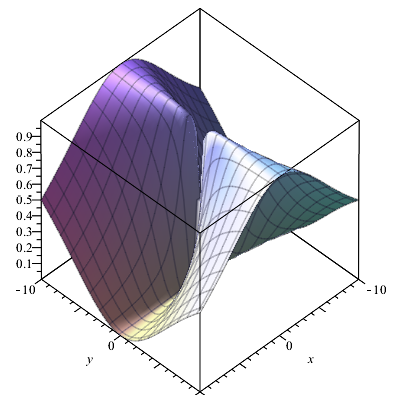
\includegraphics[width=0.6\textwidth]{plots/function4.png}
    \caption{الدالة $f(x,y)=\mfrac{y^2}{x^2+y^2}$}
    \label{fig:y2_x2y2}
\end{figure}

\begin{example}
    اثبت أن الدالة
    \[
    f(x,y)=\begin{cases}
        (x^2+y^2)\sin{\dfrac{1}{\sqrt{x^2+y^2}}}&(x,y)\neq(0,0)\\
        0&(x,y)=(0,0)
    \end{cases}
    \]
    قابلة للاشتقاق على $\R^2$ ولكنها قابلة للاشتقاق بصورة غير مستمرة عند $(0,0)$.
\end{example}
\begin{myproof}
    عندما $(x,y)\neq(0,0)$ $\Leftarrow$ $f_x$ و $f_y$ موجودة و مستمرة مع :
    \[
    f_x(x,y)=\frac{-x}{\sqrt{x^2+y^2}}\cos\dfrac{1}{\sqrt{x^2+y^2}}+2x\sin{\dfrac{1}{\sqrt{x^2+y^2}}}
    \]
    \[
    f_y(x,y)=\frac{-y}{\sqrt{x^2+y^2}}\cos\dfrac{1}{\sqrt{x^2+y^2}}+2y\sin{\dfrac{1}{\sqrt{x^2+y^2}}}
    \]
    إذن $f$ قابلة للاشتقاق على $\R^2\textbackslash\cbracket{(0,0)}$. الآن بما أن $f_x(x,0)$ ليس لها غاية عندما $x\to0$ $\Leftarrow$ $f_x$ ليست مستمرة عند $(0,0)$. لايجاد $f_x(0,0)$ نستخدم التعريف
\[
f_x(0,0)=\lim\limits_{h\to0}\frac{f(h,0)-f(0,0)}{h}=\lim\limits_{h\to0}h\sin\dfrac{1}{\abs{h}}=0
\]
بنفس الطريقة نجد أن $f_y(0,0)=0$ وبالتالي $\nabla f(0,0)=(0,0)$ ، لاثبات أن $f$ قابلة للاشتقاق عند $(0,0)$ نستخدم التعريف \eqref{eq:differentiability_second_eq}
\[
\frac{f(h,k)-f(0,0)-\nabla f(0,0)\cdot(h,k)}{\norm{(h,k)}}=\sqrt{h^2+k^2}\sin{\dfrac{1}{\sqrt{h^2+k^2}}}\to0
\]
عندما $(h,k)\to(0,0)$ إذن $f$ قابلة للاشتقاق عند $(0,0)$. (أنظر شكل \ref{fig:x2y2sinx2y2})
\end{myproof}
\begin{figure}[ht]
    \centering
    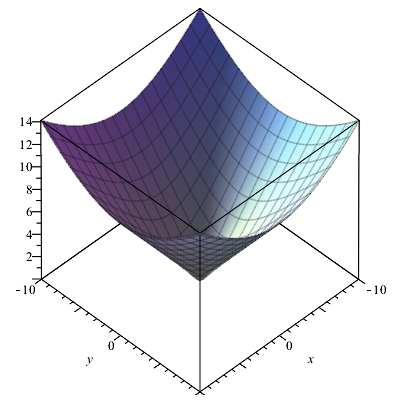
\includegraphics[width=0.6\textwidth]{plots/function3.png}
    \caption{الدالة $f(x,y)=(x^2+y^2)\sin\mfrac{1}{\sqrt{x^2+y^2}} $}
    \label{fig:x2y2sinx2y2}
\end{figure}
\begin{example}
    أثبت أن الدالة $f(x,y)=\sqrt{\abs{xy}}$ غير قابلة للاشتقاق عند النقطة $(0,0)$.
\end{example}
\begin{myproof}
    أولاً نجد المشتقات الجزئية عند $(0,0)$ 
    \[
    f_x(0,0)=\lim\limits_{h\to0}\frac{f(h,0)-f(0,0)}{h}=\lim\limits_{h\to0}\frac{0-0}{h}=0
    \]
    \[
    f_y(0,0)=\lim\limits_{k\to0}\frac{f(0,k)-f(0,0)}{k}=\lim\limits_{k\to0}\frac{0-0}{k}=0
    \]
إذن المشتقات الجزئية موجودة عند $(0,0)$ ومنه $\nabla f(0,0)=(0,0)$. الآن نستخدم التعريف لتحديد قابلية الاشتقاق
\[
\frac{f(h,k)-f(0,0)-\nabla f(0,0)\cdot (h,k)}{\norm{(h,k)}}=\frac{\sqrt{\abs{hk}}}{\sqrt{h^2+k^2}}
\]
وعند أخذ الغاية عندما $(h,k)\to(0,0)$ نلاحظ الاقتراب على المسار $k=0$ يعطي
\[
\lim\limits_{(h,k)\to(0,0)}\frac{\sqrt{\abs{hk}}}{\sqrt{h^2+k^2}}=\lim\limits_{h\to0}\frac{0}{\sqrt{h^2}}=0
\]
أما الاقتراب على المسار $h=k$ يعطي
\[
\lim\limits_{(h,k)\to(0,0)}\frac{\sqrt{\abs{hk}}}{\sqrt{h^2+k^2}}=\lim\limits_{h\to0}\frac{\sqrt{\abs{h^2}}}{\sqrt{2h^2}}=\lim\limits_{h\to0}\frac{\abs{h}}{\sqrt{2}\abs{h}}=\frac{1}{\sqrt{2}}
\]
إذن الغاية غير موجودة وبالتالي الدالة $f$ ليست قابلة للاشتقاق عند $(0,0)$. (أنظر شكل \ref{fig:sqrt_xy})
\end{myproof}
\begin{figure}[ht]
    \centering
    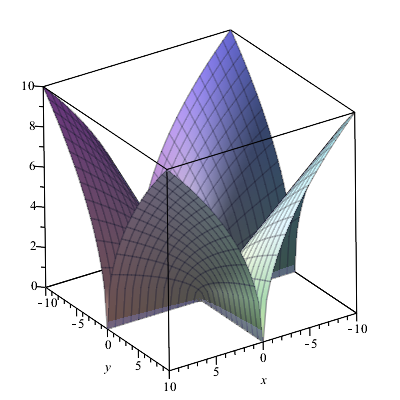
\includegraphics[width=0.6\textwidth]{plots/function5.png}
    \caption{الدالة $f(x,y)=\sqrt{xy}$}
    \label{fig:sqrt_xy}
\end{figure}

\begin{example}
    أثبت أن الدالة 
    \[
    f(x,y)=\begin{cases}
        \dfrac{x^2-2y^2}{1-\cos{\sqrt{x^2-3y^2}}} & 0<\norm{(x,y)}<\pi\\
        0&(x,y)=(0,0)
    \end{cases}
    \]
    غير قابلة للاشتقاق عند النقطة $(0,0)$.
\end{example}
\begin{myproof}
    نجد المشتقة الجزئية بالنسبة إلى $x$ عند $(0,0)$
    \begin{align*}
    f_x(0,0)&=\lim\limits_{h\to0}\frac{f(h,0)-f(0,0)}{h}\\[7pt]
    &=\lim\limits_{h\to0}\frac{1}{h}\cdot\frac{h^2-0}{1-\cos{\sqrt{h^2-0}}}\\[7pt]
    &=\lim\limits_{h\to0}\frac{h}{1-\cos\abs{h}}
    \end{align*}
    وهذه الغاية غير موجودة وبالتالي $f_x(0,0)$ غير موجودة $\Leftarrow$ الدالة $f$ غير قابلة للاشتقاق عند $(0,0)$.
\end{myproof}
%\section{التفاضل في $\R^n$}
\begin{theorem}
    لتكن $\alpha\in\R$, $\A\in\R^n$ و أن $\f,\g$ دوال إتجاهية فإذا كان كل من $\f$ و $\g$ دوال قابلة للإشتقاق عند $\A$ فإن $\f+\g$ , $\alpha\f$ و $\f\cdot\g$ كلها دوال قابلة للإشتقاق عند $\A$. في الحقيقة
    \begin{align}
        &D(\f+\g)(\A)=D\f(a)+D\f(b)\\
        &D(\alpha\f)(\A)=\alpha D\f(\A)
    \end{align}
    و
\begin{equation}
    D(\f\cdot\g)(\A)=\g(\A)D\f(\A)+\f(\A)D\g(\A)
\end{equation}
\end{theorem}

\begin{example}
    إثبت أن الدوال الإتجاهية التالية قابلة للإشتقاق في مجالها ومن ثم أوجد $D(\f+\g)(\x)$ و $D(\f\cdot\g)(\x)$.\\[5pt]
    (a) $\f(x,y)=2x-4y,\quad \g(x,y)=2x^2+y^3$\\[5pt]
    (b) $\f(x,y,z)=(-y,x+z),\quad \g(x,y,z)=(x+y+z,xyz)$
\end{example}
\begin{solution}
(a) نجد المشتقات
\[
\f_x=2,\,\f_y=-4\quad \g_x=4x,\,\g_y=3y^2
\] 
المجال هو $\R^2$. نلاحظ أن المشتقات الجزئية موجودة و مستمرة عند جميع نقاط $\R^2$ بالتالي فإن $\f,\g$ دوال قابلة للإشتقاق على $\R^2$. الآن
\begin{align*}
   & D\f=\begin{bmatrix}
        \f_x&\f_y
    \end{bmatrix}=\begin{bmatrix}
        2&-4
    \end{bmatrix}\\
   & D\g=\begin{bmatrix}
        \g_x&\g_y
    \end{bmatrix}=\begin{bmatrix}
        4x&3y^2
    \end{bmatrix}
\end{align*}
إذن
\[
D(\f+\g)=D\f+D\g=\begin{bmatrix}
    2+4x&-4+3^2
\end{bmatrix}
\]
كذلك
\begin{align*}
    D(\f\cdot\g(\x)&=\g(\x)D\f(\x)+\f(\x)D\g(\x)\\
    &=(2x^2+y^3)\begin{bmatrix}
        2&-4
    \end{bmatrix}+(2x-4y)\begin{bmatrix}
        4x&3y^2
    \end{bmatrix}\\
    &=\begin{bmatrix}
        4x^2+2y^3&-8x^2-4y^3
    \end{bmatrix}+\begin{bmatrix}
        8x^2-16xy&6xy-12y^3
    \end{bmatrix}\\
    &=\begin{bmatrix}
        12x^2+2y^3-16xy&-16y^3-8x^2+6xy^2
    \end{bmatrix}
\end{align*}
(b) المجال هو جميع نقاط $\R^3$. نجد المشتقات 
\begin{align*}
   & \f_x=(0,1),\,\f_y=(-1,0),\,\f_z=(0,1)\\
   & \g_x=(1,yz),\,\g_y=(1,xz),\,\g_z=(1,xy)
\end{align*}
المشتقات الجزئية جميعها موجودة و مستمرة عند جميع نقاط $\R^3$ إذن كل من $\f,\g$ دوال قابلة للإشتقاق على $\R^3$. الآن
\begin{align*}
   & D\f=\begin{bmatrix}
        \f_x&\f_y&\f_z
    \end{bmatrix}_{2\times3}=\begin{bmatrix}
        0&-1&0\\
        1&0&1
    \end{bmatrix}\\
   & D\g=\begin{bmatrix}
        \g_x&\g_y&\g_z
    \end{bmatrix}_{2\times3}=\begin{bmatrix}
        1&1&1\\
        yz&xz&xy
    \end{bmatrix} 
\end{align*}
إذن
\[
D(\f+\g)=D\f+D\g=\begin{bmatrix}
    1&0&1\\
    1+yz&xz&1+xy
\end{bmatrix}
\]
كذلك
\begin{align*}
    D(\f\cdot\g)(\x)&=\g(\x)D\f(\x)+\f(\x)D\g(\x)\\
    &=\begin{bmatrix}
        x+y+z&xyz
    \end{bmatrix}\begin{bmatrix}
        0&-1&0\\
        1&0&1
    \end{bmatrix}+\begin{bmatrix}
        -y&x+z
    \end{bmatrix}\begin{bmatrix}
        1&1&1\\
        yz&xz&xy
    \end{bmatrix}\\
    &=\begin{bmatrix}
        -y+xyz+yz^2&-y+x^2z+xz^2&-y+x^2y+xyz
    \end{bmatrix}+\begin{bmatrix}
        xyz&-x-y-z&xyz
    \end{bmatrix}\\
    &=\begin{bmatrix}
        -y+2xyz+yz^2&xz^2+2x^2-x-2y-z&-y+x^2y+2xyz
    \end{bmatrix}
\end{align*}

\end{solution}

\begin{theorem}
    لتكن $f:\R^n\to\R$ دالة قابلة للإشتقاق عند $\A$ و $\Delta\x=(\Delta x_1,\dots,\Delta x_n)$ ، فإن
\[
\frac{\Delta z-dz}{\norm{\Delta\x}}\to0\quad\text{عندما}\quad\Delta\x\to\Bzero
\]
حيث $z=f(\x)$ و $\Delta z=f(\A+\Delta \x)-f(\A)$. بالخصوص فإن $dz$ تقريب جيد $\Delta z$.
\end{theorem}
\begin{myproof}
    بالتعريف ، إذا كانت $f$ قابلة للإشتقاق عند $\A$ ، إذن $\epsilon(\h):=f(\A+\h)-f(\A)-\nabla f(\A)\cdot\h$ يحقق $\epsilon(\h)/\norm{\h}\to\Bzero$ عندما $\h\to\Bzero$. بما أن $\Delta z=f(\A+\h)-f(\A)$ لــ $\h:=\Delta\x$ و $dz=\nabla f(\A)\cdot \h$ فإنه يبتع بأن $(\Delta z-dz)/\norm{\Delta\x}\to\Bzero$ عندما $\Delta\x\to\Bzero$.
\end{myproof}
\begin{example}
    إستخدم التفاضل لتقريب التغير في $f(x,y)=x^2y-x^3$ عندما نتحرك من $(0,1)$ إلى $(0.02,1.01)$.
\end{example}
\begin{solution}
    ليكن $z=x^2y-x^3$ , $a=0$ , $b=1$ إذن
    \begin{gather*}
        dx=0.02-0=0.02\\
        dy=1.01-1=0.01
    \end{gather*}
    الآن
    \begin{align*}
        dz&=\frac{\partial f}{\partial x}dx+\pder{f}{y}dy\\
        &=2xydx+(x^2-3y^2)dy
    \end{align*}
    ومن ثم
\begin{align*}
    \Delta z\approx dz(0,1)&=2(0)(1)(0.02)+(0^2-3(1))(0.01)\\
    &=0+(-3)(0.01)=-0.03
\end{align*}
نلاحظ أن القيمة الحقيقية $\Delta z=f(0.02,1.01)-f(0,1)=-0.29897$ قريب جداً من $-0.03$.
\end{solution}

\begin{example}
    استخدم التفاضل لتقريب المقدار $(5.97)\sqrt[4]{16.03}$
\end{example}
\begin{solution}
    ليكن $z=y\sqrt[4]{x}$ , $a=16$ ,$b=6$ إذن
    \[
    dx=16.03-16=0.03,\quad dy=5.97-6=-0.03
    \]
    ومن ثم
\begin{align*}
    dz&=\pder{f}{x}dx+\pder{f}{y}dy\\
   & =\frac{y}{4\sqrt[4]{x^3}}dx+\sqrt[4]{x}dy
\end{align*}
إذن
\[
\Delta z\approx\frac{6(0.03)}{4\sqrt[4]{16^3}}+\sqrt[4]{16}(-0.03)=-0.054375
\]
ومنه
\[
z\approx 6\sqrt[4]{16}-0.059375=11.945625
\]
القيمة الحقيقية هي $11.945593$ إذن التقريب جيد إلى ثلاث مراتب عشرية.
\end{solution}